% Drawing 156-7/05-2 -- folder 156-7, batch 05, archive page 82 (PDF page 83).
% Transcription: dessin à gauche : un fuseau de $0$ à $1$ ; sur l'arc supérieur les points $x_1$, $(x_3)$, $x_2$, sur l'arc inférieur $x'_2$, $(x'_3)$, $x'_1$ ; les segments $[x_1, x_2]$ et $[x'_2, x'_1]$ sont repassés en gras ; à côté, « $z_1 = (x_1, x'_1)$ », « $z_2 = (x_2, x'_2)$ »
% Kind: spindle with marked points. Method 2 (schematic redraw from the facsimile). Status: ok.
% Notes: Spindle from 0 to 1; on the upper arc x_1, (x_3), x_2, on the lower arc x'_2, (x'_3), x'_1; the segments [x_1, x_2] and [x'_2, x'_1] thick; on the left z_1 = (x_1, x'_1), z_2 = (x_2, x'_2). The formula under the drawing belongs to the text.
% Coordinates: 1 unit = 1 mm = 1/100 of the crop width (bbox in page fractions: [0.08, 0.76, 0.45, 0.86]).
% Redrawn by Claude (claude-opus-5-5), issue #73, 2026-11-07; not checked by a human; not compiled (no TeX in the session).
% Rights: reproduces part of the work -- behind RENDER_TRANSCRIPTS, never published by itself.
\documentclass[tikz,border=3pt]{standalone}
\usepackage{amsmath,amssymb}
\usetikzlibrary{patterns,arrows.meta}
\tikzset{pencil/.style={black!45}, struck/.style={black!35}, mark/.style={circle,draw,inner sep=1.3pt}, pt/.style={circle,fill,inner sep=0.9pt}, opt/.style={circle,draw,fill=white,inner sep=1.1pt}}
\begin{document}
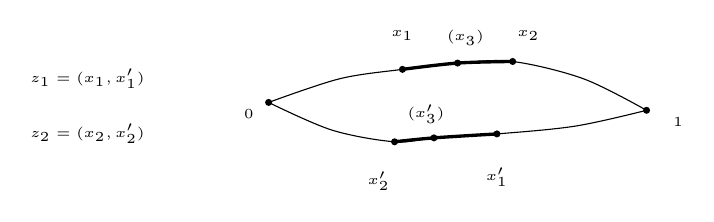
\begin{tikzpicture}[x=1mm,y=1mm,line cap=round,line join=round,font=\scriptsize]
\draw plot[smooth, tension=0.55] coordinates {(37,-15) (46,-12) (54,-10.8) (61,-10) (68,-9.8) (77,-12) (85,-16)};
\draw plot[smooth, tension=0.55] coordinates {(37,-15) (45,-18.5) (53,-20) (58,-19.5) (66,-19) (76,-18) (85,-16)};
\draw[very thick] plot[smooth, tension=0.55] coordinates {(54,-10.8) (61,-10) (68,-9.8)};
\draw[very thick] plot[smooth, tension=0.55] coordinates {(53,-20) (58,-19.5) (66,-19)};
\node[pt] at (37,-15) {};
\node[pt] at (85,-16) {};
\node[pt] at (54,-10.8) {};
\node[pt] at (61,-10) {};
\node[pt] at (68,-9.8) {};
\node[pt] at (53,-20) {};
\node[pt] at (58,-19.5) {};
\node[pt] at (66,-19) {};
\node[inner sep=1pt] at (34.5,-16.5) {\tiny $0$};
\node[inner sep=1pt] at (89,-17.5) {\tiny $1$};
\node[inner sep=1pt] at (54,-6.5) {\tiny $x_1$};
\node[inner sep=1pt] at (62,-6.8) {\tiny $(x_3)$};
\node[inner sep=1pt] at (70,-6.5) {\tiny $x_2$};
\node[inner sep=1pt] at (51,-25) {\tiny $x'_2$};
\node[inner sep=1pt] at (57,-16.5) {\tiny $(x'_3)$};
\node[inner sep=1pt] at (66,-24.5) {\tiny $x'_1$};
\node[inner sep=1pt] at (14,-12) {\tiny $z_1=(x_1,x'_1)$};
\node[inner sep=1pt] at (14,-19) {\tiny $z_2=(x_2,x'_2)$};
\end{tikzpicture}
\end{document}
